% Séquence 1 : Enchaînement d'opérations
\setseqtitle{Enchaînement d'opérations}
\chapter{Enchaînement d'opérations}

\begin{objectifsbox}
\textbf{Objectifs d'apprentissage.} À l'issue de la séquence, l'élève sera capable de :
\begin{itemize}
\item Calculer des expressions avec plusieurs opérations en respectant les priorités
\item Utiliser les parenthèses pour modifier l'ordre des calculs
\item Identifier la nature d'une expression (somme, produit, quotient)
\item Utiliser le vocabulaire mathématique approprié
\end{itemize}
\end{objectifsbox}

\section{Calculer sans parenthèses}

\subsection{Activité d'introduction}

\begin{activitybox}
Voici trois calculs effectués à la calculatrice :

\begin{center}
\begin{tabular}{|c|c|}
\hline
\textbf{Expression} & \textbf{Résultat} \\
\hline
$8 \div 2 \times 5$ & $20$ \\
\hline
$6 \times 2 \div 3$ & $4$ \\
\hline
$24 \div 6 \div 2$ & $2$ \\
\hline
\end{tabular}
\end{center}

\begin{enumerate}[label=\alph*)]
\item Pour chaque calcul, entourer en rouge l'opération qui a été effectuée en premier par la calculatrice.
\item Calculer mentalement l'expression numérique $10 \div 5 \times 2$
\end{enumerate}
\end{activitybox}

\subsection{Règles de calcul sans parenthèses}
\begin{proprietebox}
\begin{itemize}[label = \textbullet]
\item Dans une expression sans parenthèses, ne comportant que des \textbf{additions et des soustractions}, on effectue les calculs de la gauche vers la droite.
\item Dans une expression sans parenthèses, ne comportant que des \textbf{multiplications et des divisions}, on effectue les calculs de la gauche vers la droite.
\end{itemize}
\end{proprietebox}

\begin{examplebox}
\textbf{Exemple :} Calculer les expressions A et B en détaillant les calculs.

\begin{minipage}[t]{0.48\textwidth}
\begin{align*}
A &= 16 - 12 + 7 + 5 - 8 \\
&= \trous{4cm} \\
&= \trous{3cm} \\
&= \trous{2cm} \\
&= \trous{1cm}
\end{align*}
\end{minipage}
\hfill
\begin{minipage}[t]{0.48\textwidth}
\begin{align*}
B &= 40 \div 8 \times 2 \\
&= \trous{4cm} \\
&= \trous{3cm}
\end{align*}
\end{minipage}
\end{examplebox}

\subsection{Priorités opératoires}
\begin{proprietebox}
Dans une expression sans parenthèses, on effectue d'abord les \textbf{multiplications et les divisions}, puis les \textbf{additions et les soustractions}. 

On dit que la multiplication et la division sont \textbf{prioritaires} par rapport à l'addition et à la soustraction.
\end{proprietebox}

\begin{examplebox}
Calculer les expressions C et D en détaillant les calculs.

\begin{minipage}[t]{0.48\textwidth}
\begin{align*}
C &= 23 + 6 \times 4 \\
&= \trous{3cm} \\
&= \trous{3cm}
\end{align*}
\end{minipage}
\begin{minipage}[t]{0.48\textwidth}
\begin{align*}
D &= 7 \times 8 - 12 \div 4 \\
&= \trous{3cm} \\
&= \trous{3cm}
\end{align*}
\end{minipage}
\end{examplebox}

\section{Calculer avec parenthèses}

\begin{proprietebox}
\begin{itemize}[label = \textbullet]
\item Dans une expression avec des parenthèses, on effectue d'abord les calculs \textbf{entre parenthèses}.
\item Quand il y a plusieurs niveaux de parenthèses, on commence par les \textbf{plus intérieures}.
\item À l'intérieur des parenthèses, on applique les \textbf{priorités de calcul}.
\end{itemize}
\end{proprietebox}

\begin{examplebox}
Calculer les expressions E, F et G en détaillant les calculs.

\begin{minipage}[t]{0.32\textwidth}
\begin{align*}
E &= 9 \times (7 + 4) \\
&= \trous{3cm} \\
&= \trous{3cm}
\end{align*}
\end{minipage}
\hfill
\begin{minipage}[t]{0.32\textwidth}
\begin{align*}
F &= 2,5 \times [7 - (5 - 3)] \\
&= \trous{3cm}\\
&= \trous{3cm}\\
&= \trous{3cm}
\end{align*}
\end{minipage}
\hfill
\begin{minipage}[t]{0.32\textwidth}
\begin{align*}
G &= 12 \times (5 + 2 \times 3) \\
&= \trous{3cm} \\
&= \trous{3cm} \\
&= \trous{3cm}
\end{align*}
\end{minipage}
\end{examplebox}

\begin{remarkbox}
\begin{itemize}[label = \textbullet]
\item Les parenthèses changent l'ordre des calculs et donc le résultat.
\item Les parenthèses disparaissent lorsque les calculs à l'intérieur sont achevés.
\end{itemize}
\end{remarkbox}

\section{Calculer avec un quotient}

\begin{proprietebox}
Une expression qui figure au numérateur ou au dénominateur d'un quotient est considérée comme \textbf{entre parenthèses}.
\end{proprietebox}

\begin{examplebox}
Calculer les expressions H et I en détaillant les calculs.

\begin{minipage}{0.48\textwidth}
\textbf{H = $\frac{9 + 5}{7}$}

H peut aussi s'écrire : $(9 + 5) \div 7$

\begin{align*}
H &= \frac{9 + 5}{7} \\
&= \trous{3cm} \\
&= \trous{3cm}
\end{align*}
\end{minipage}
\hfill
\begin{minipage}{0.48\textwidth}
\textbf{I = $\frac{20}{8 - 3}$}

I peut aussi s'écrire : $20 \div (8 - 3)$

\begin{align*}
I &= \frac{20}{8 - 3} \\
&= \trous{3cm} \\
&= \trous{3cm}
\end{align*}
\end{minipage}
\end{examplebox}

\section{Utiliser le bon vocabulaire}
\begin{definitionbox}
\begin{itemize}[label = \textbullet]
\item Le résultat d'une \textbf{addition} est une \textbf{somme}. Les nombres additionnés sont les \textbf{termes}.
\item Le résultat d'une \textbf{soustraction} est une \textbf{différence}. Les nombres qui interviennent dans la soustraction sont les \textbf{termes}.
\item Le résultat d'une \textbf{multiplication} est un \textbf{produit}. Les nombres multipliés sont les \textbf{facteurs}.
\item Le résultat d'une \textbf{division} est un \textbf{quotient}.
\end{itemize}
\end{definitionbox}

\begin{examplebox}
\begin{center}
	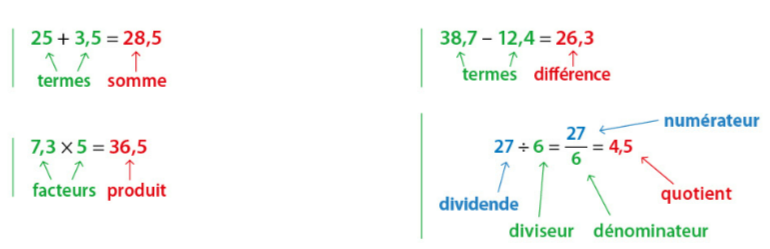
\includegraphics[width=1\linewidth]{../../assets/images/6e/seq_01/vocabualire_operations}
\end{center}
\end{examplebox}

\begin{definitionbox}
La nature d'une expression comportant plusieurs opérations est déterminée par l'opération effectuée en dernier.
\end{definitionbox}

\begin{examplebox}
Dans l'expression $2 + 3 \times 5$, c'est \trous{5cm} qu'on effectue en dernier, car la \trous{5cm} est prioritaire. Cette expression est donc une \trous{5cm}. C'est \trous{5cm} de $2$ et du \trous{5cm} de $3$ par $5$.
\end{examplebox}

\section{Exercices d'application}
\begin{exercisebox}
\textbf{Exercice 1 :} Calculer les expressions suivantes en détaillant les calculs.

\begin{enumerate}[label=\alph*)]
\item $A = 15 + 8 \times 3$
\item $B = 24 \div 6 + 5 \times 2$
\item $C = 10 - 3 \times 2 + 7$
\item $D = 18 \div (6 - 3) \times 4$
\end{enumerate}

\textbf{Exercice 2 :} Calculer les expressions suivantes.

\begin{enumerate}[label=\alph*)]
	\item $E = \frac{12 + 8}{5}$
	\item $F = \frac{30}{6 - 1}$
	\item $G = 5 \times (3 + 2 \times 4)$
	\item $H = [10 - (4 + 1)] \times 3$
\end{enumerate}

\textbf{Exercice 3 :} Identifier la nature de chaque expression (somme, différence, produit ou quotient).

\begin{enumerate}[label=\alph*)]
	\item $7 + 3 \times 2$
	\item $15 \div 3 + 4$
	\item $8 \times (5 - 2)$
	\item $\frac{20 + 4}{6}$
\end{enumerate}
\end{exercisebox}


